\chapter{Laboratorio 1}
In questa esperienza di laboratorio si è realizzato e analizzato il seguente circuito:
\begin{figure}[h!]
	\begin{minipage}{.4\textwidth}
	\begin{circuitikz}[scale=.9, use fpu reciprocal]
		\draw (0,.5) node[ground]{} coordinate(botl);
		\draw (0,2) to[sV=$v_{in}$] (0,.5);
		\draw (0,2) to[R=$R_2$, -*] ++(3,0) ++(0.1,-.1) node[below]{$V^-$};
		\draw (3,2) to (4,2);
		\draw (3.7,2) node[op amp, anchor=-](oa){\texttt{TL071}};
		\draw (3.7,.5) node[ground]{} to[short, -*] (3.7,.9);
		\draw (3,2) -- ++(0,1.3) coordinate(C) to[C=$C_1$] ++(3.35,0) (C-|oa.out) coordinate(Co) -- (oa.out) to [short, *-o] ++(1,0) node[above]{$v_{out}$} coordinate(maxr);
		\draw (3,3.3) -- ++(0,1.3) to[R=$R_1$] ++(3,0) -| (Co);
		\draw[thick] (-.7,-.5) rectangle (7.7,5.5); % the frame
	\end{circuitikz}
	\end{minipage}
	\qquad\qquad
	\begin{minipage}{.463\textwidth}
		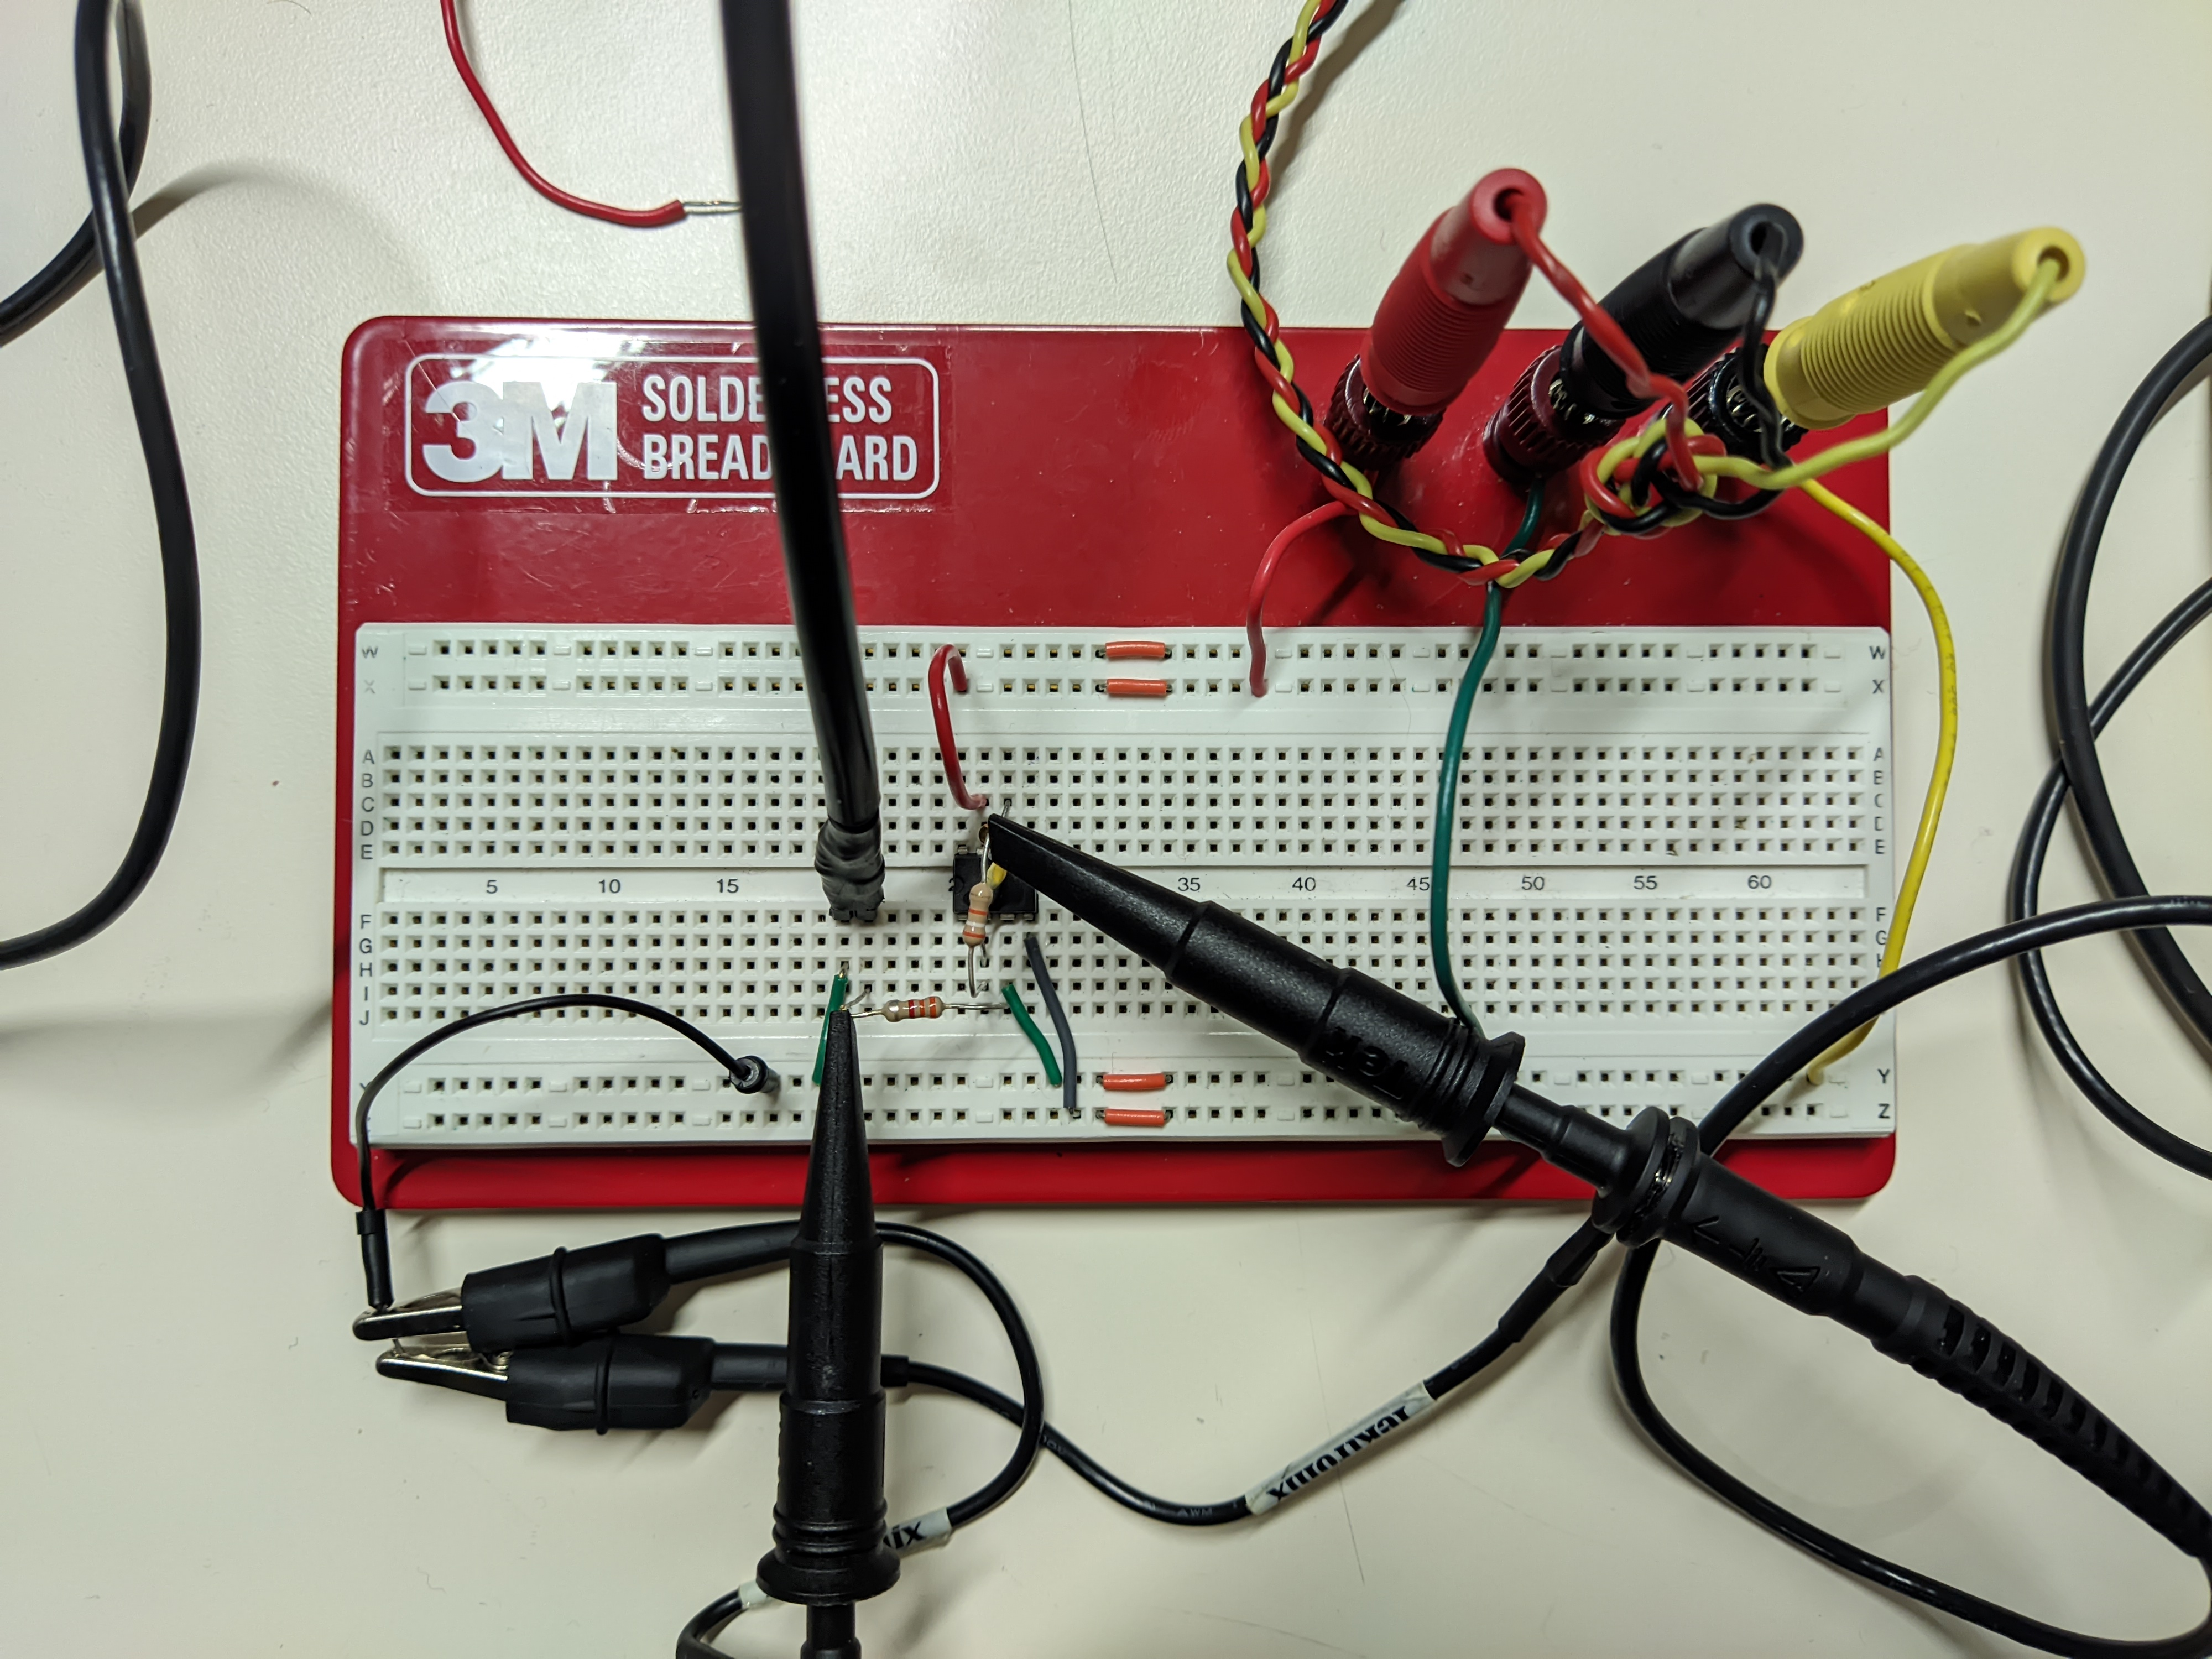
\includegraphics[width=\linewidth]{./ImageFiles/Laboratorio 1/CIRC.jpg}
	\end{minipage}
	\caption{Schema circuitale e foto circuito}
	\label{fig:circuito}
\end{figure}

Il circuito realizza un filtro passa basso attivo, utilizzando un amplificatore operazionale retroazionato negativamente. Infatti, è possibile ricavare la funzione di trasferimento del circuito tramite un bilancio delle correnti al nodo V\super{-}. Si consideri v\sub{in} come un generatore ideale di tensione applicato in ingresso al circuito. Indicando con Z\sub{1} l'impedenza equivalente del parallelo tra R\sub{1} e C\sub{1} e con Z\sub{2} l'impedenza della resistenza R\sub{2}, si può ottenere la funzione di trasferimento del circuito:
\begin{equation}
	v_{out}=-\frac{Z_1}{Z_2}v_{in}=-\frac{1}{R_2}\frac{R_1}{1+j w R_1 C_1} vin,
\end{equation}
da cui si ricava
\begin{equation}
	T=\frac{v_{out}}{v_{in}}=-\frac{R_1}{R_2}\frac{1}{1+j w R_1 C_1}.
\end{equation}
Questa funzione di trasferimento corrisponde a un filtro passa basso. Infatti, è possibile calcolare l'espressione del modulo e della fase in funzione di $\omega$:
\begin{equation}
	\begin{split}
		|T|&=\frac{R_1}{R_2}\frac{1}{\sqrt{1+(wR_1C_1)^2}} \\
		\angle T&=\SI{180}{\degree}-arctan(\omega R_1 C_1).
	\end{split}
\end{equation}
Per comprendere l'andamento del modulo e della fase in funzione della frequenza del segnale applicato in ingresso, è necessario analizzare i termini dipendenti da $\omega$ nelle due equazioni. Nell'espressione del modulo della funzione di trasferimento, il termine 
\begin{equation}
	\sqrt{1+(wR_1C_1)^2} \to
	\begin{cases}
		1 \; per \; \omega \to 0 \\
		\infty \; per \; \omega \to \infty
	\end{cases}
,
\end{equation}
mentre nell'espressione della fase, il termine
\begin{equation}
	arctan(\omega R_1 C_1) \to
	\begin{cases}
		0 \; per \; \omega \to 0 \\
		90^\circ \; per \; \omega \to \infty
	\end{cases}
	.
\end{equation}


Il modulo quindi tende a $\frac{R_1}{R_2}$ per segnali in ingresso a bassa frequenza, mentre tende a zero per segnali in ingresso ad alta frequenza, mentre la fase è pari a circa \SI{180}{\degree} per segnali a bassa frequenza, e tende a \SI{90}{\degree} per segnali ad alta frequenza.\todo{da sistemare questa parte}
Si determina quindi un comportamento di un filtro passa basso invertente del primo ordine, con frequenza di taglio pari a $f=\frac{1}{2\pi R_1C_1}$.

I valori dei componenti passivi sono stati scelti per soddisfare i requisiti di prestazioni del filtro. In particolare, veniva richiesto un guadagno di un fattore 10 con frequenza di taglio pari a \SI{10}{\kilo\hertz}. I valori scelti ... (\todo{inserire tabella valori con valori nominali/misurati dei componenti}).

\todo{Inserire grafici matlab}
\todo{inserire prove di saturazione}
\todo{inserire prove di offset}
